\documentclass{urdpl}     % praca w języku polskim

% Lista wszystkich języków stanowiących języki pozycji bibliograficznych użytych w pracy.
% (Zgodnie z zasadami tworzenia bibliografii każda pozycja powinna zostać utworzona zgodnie z zasadami języka, w którym dana publikacja została napisana.)
\usepackage[english,polish]{babel}

% Użyj polskiego łamania wyrazów (zamiast domyślnego angielskiego).
\usepackage{polski}

\usepackage[utf8]{inputenc}

% dodatkowe pakiety

\usepackage{mathtools}
\usepackage{amsfonts}
\usepackage{amsmath}
\usepackage{amsthm}
\usepackage[hidelinks]{hyperref}
\usepackage{float}
\usepackage{listings}
\usepackage{graphicx}
\usepackage{subcaption}
\usepackage{booktabs} % Dla \toprule, \midrule, \bottomrule
\usepackage{multirow} 
\usepackage{tabularx} 
\usepackage{amssymb} 
\usepackage{listings}
\usepackage{xcolor}
\usepackage{array}
\usepackage{makecell}
\usepackage[flushleft]{threeparttable}
\usepackage[normalem]{ulem}
\usepackage{lineno}
% ---------------------------------------------

% --- < bibliografia > ---

\usepackage{csquotes}

% ------------------------
% --- < listingi > ---

% Użyj czcionki kroju Courier.
\usepackage{courier}

\usepackage{listings}
\lstloadlanguages{TeX}
\renewcommand{\lstlistlistingname}{Spis listingów}
\renewcommand{\lstlistingname}{Listing}


\lstset{
	literate={ą}{{\k{a}}}1
           {ć}{{\'c}}1
           {ę}{{\k{e}}}1
           {ó}{{\'o}}1
           {ń}{{\'n}}1
           {ł}{{\l{}}}1
           {ś}{{\'s}}1
           {ź}{{\'z}}1
           {ż}{{\.z}}1
           {Ą}{{\k{A}}}1
           {Ć}{{\'C}}1
           {Ę}{{\k{E}}}1
           {Ó}{{\'O}}1
           {Ń}{{\'N}}1
           {Ł}{{\L{}}}1
           {Ś}{{\'S}}1
           {Ź}{{\'Z}}1
           {Ż}{{\.Z}}1,
	basicstyle=\footnotesize\ttfamily,
}

% defninicja stylu python
\lstdefinestyle{stylePython}{
    language=Python,
    commentstyle=\color{green},          % Kolor komentarzy
    keywordstyle=\color{blue},           % Kolor słów kluczowych
    numberstyle=\tiny\color{gray},       % Kolor i styl numerów linii
    stringstyle=\color{red},             % Kolor ciągów znaków
    basicstyle=\ttfamily\footnotesize,   % Podstawowy styl kodu
    breakatwhitespace=false,             % Automatyczne dzielenie wierszy
    breaklines=true,                     % Dzielenie długich linii
    keepspaces=true,                     % Zachowanie spacji
    numbers=left,                        % Numery linii po lewej
    numbersep=5pt,                       % Odstęp numerów od kodu
    showspaces=false,                    % Nie pokazuj spacji
    showstringspaces=false,              % Nie pokazuj spacji w ciągach znaków
    showtabs=false,                      % Nie pokazuj tabulacji
    tabsize=2                            % Rozmiar tabulacji
}

% defnicja stylu JAVA
\lstdefinestyle{javaStyle}{
    language=Java,
    basicstyle=\ttfamily\footnotesize,
    keywordstyle=\color{blue},
    commentstyle=\color{green!50!black}\itshape,
    stringstyle=\color{green},
    numberstyle=\tiny\color{gray},
    numbers=left,
    numbersep=5pt,                       % Odstęp numerów od kodu
    stepnumber=1,
    showspaces=false,                    % Nie pokazuj spacji
    tabsize=2,
    showstringspaces=false,
    breaklines=true,
    breakatwhitespace=false,             % Automatyczne dzielenie wierszy
    showtabs=false,                      % Nie pokazuj tabulacji
    keepspaces=true                    % Zachowanie spacji
}


\definecolor{stringcolor}{RGB}{163,21,21}    % pomarańczowy - stringi
\definecolor{typecolor}{RGB}{43, 145, 176}     % ciemny fiolet - klasy, typy

\lstdefinestyle{csStyle}{
    language=[Sharp]C, % dla C#; można zmienić na Java
    basicstyle=\ttfamily\footnotesize,
    keywordstyle=\color{blue},
    stringstyle=\color{stringcolor},
    commentstyle=\color{green!50!black}\itshape,
    morekeywords={class, public, private, protected, static, void, string, int, new}, % dodatkowe słowa kluczowe
    emphstyle=\color{typecolor}\bfseries, % klasy na fioletowo
    numbers=left,
    numbersep=5pt,                       % Odstęp numerów od kodu
    numberstyle=\tiny\color{gray},
    stepnumber=1,
    breaklines=true,
    showspaces=false,                    % Nie pokazuj spacji
    tabsize=2,
    showstringspaces=false,
    breakatwhitespace=false,             % Automatyczne dzielenie wierszy
    showtabs=false,                      % Nie pokazuj tabulacji
    keepspaces=true                    % Zachowanie spacji  
}

\definecolor{lightgray}{rgb}{0.9,0.9,0.9}
    % \definecolor{blue}{rgb}{0,0,1}
    \definecolor{green}{rgb}{0,0.6,0}
    % \definecolor{red}{rgb}{0.6,0,0}
    \definecolor{gray}{rgb}{0.5,0.5,0.5}

% % ------------------------
\AtBeginDocument{
	\renewcommand{\tablename}{Tabela}
	\renewcommand{\figurename}{Rys.}   
    \newcommand{\listingname}{Listing}
}


% ------------------------
% --- < tabele > ---

% defines the X column to use m (\parbox[c]) instead of p (`parbox[t]`)
\newcolumntype{C}[1]{>{\hsize=#1\hsize\centering\arraybackslash}X}

%---------------------------------------------------------------------------

\author{Kamil Kopczyk}
\shortauthor{K. Kopczyk}
\noAlbum{134927}

\titlePL{Projekt i implementacja systemu do rezerwacji usług łowiska wędkarskiego z wykorzystaniem bazy danych MySQL i języka JAVA}
\titleEN{Design and implementation of a system for booking fishing grounds services using the MySQL database and JAVA language}

\shorttitlePL{Projekt i implementacja systemu do rezerwacji usług łowiska wędkarskiego} % skrócona wersja tytułu jeśli jest bardzo długi
\shorttitleEN{Design and implementation of a system for booking fishing grounds services using the MySQL database and JAVA language}

\thesistype{Praca projektowa}


\thesisDone{Praca wykonana pod kierunkiem}
\supervisor{mgr inż. Ewa Żesławska}
%\supervisor{Ewa Żesławska PhD}

\degreeprogramme{Informatyka}
%\degreeprogramme{Computer Science}

\date{2025}

\department{Instytut Informatyki}
%\department{Institute of Computer Science}

\faculty{Wydział Nauk Ścisłych i Technicznych}
%\faculty{Faculty of Science and Technology}



\setlength{\cftsecnumwidth}{10mm}

%---------------------------------------------------------------------------
\setcounter{secnumdepth}{4}
\brokenpenalty=10000\relax

% --------------------------------------------------------------------------
% główna część pracy
% --------------------------------------------------------------------------

\begin{document}

\titlepages

% Ponowne zdefiniowanie stylu `plain`, aby usunąć numer strony z pierwszej strony spisu treści i poszczególnych rozdziałów.
\fancypagestyle{plain}
{
    % Usuń nagłówek i stopkę
    \fancyhf{}
    % Usuń linie.
    \renewcommand{\headrulewidth}{0pt}
    \renewcommand{\footrulewidth}{0pt}
}

\setcounter{tocdepth}{2}
\tableofcontents
\clearpage


% dodanie poszczególnych rozdziałów 

\chapter{Streszczenie}
\label{chap:nowe_wprowadzenie}

\section{Streszczenie w języku polskim}
Celem projektu było stworzenie systemu do rezerwacji usług łowiska wędkarskiego. Aplikacja składa się z formularzu logowania i formularza rejestracji który pozwala utworzyć konto do którego są przypisywane rezerwacje później logować się na nie rezerwować łowiska, wynajmować wędki, domki i przeglądać historię rezerwacji.System został napisany w języku \textbf{Java}, jego interfejs graficzny powstał przy użyciu biblioteki \textbf{Swing}, a za przechowywanie danych odpowiada baza \textbf{MySQL}. 

\section{Summary in English}
The aim of the project was to create a system for booking fishing grounds services. The application consists of a login form and a registration form that allows you to create an account to which reservations are assigned, then log in to them, book fishing grounds, rent fishing rods, cottages and view the history of reservations. The system was written in \textbf{Java}, its graphical interface was created using the \textbf{Swing} library, and the \textbf{MySQL} database is responsible for storing data.
\chapter{Opis założeń projektu}
\label{chap:opis}


\section*{Cele projektu}
Celem projektu było stworzenie systemu do rezerwacji usług łowiska wędkarskiego, plan zakładał budowę aplikacji która zapewni prostą obsługę rezerwacji łowisk, wędek i domków po przez proste schludne GUI jak i przeglądanie historii rezerwacji. Całość ma ułatwić i w pewnym sensie zautomatyzować
obsługę kompleksu łowisk na tyle że klient tylko przyjeżdża odbiera swoją rezerwację i idzie się cieszyć wędkowaniem bez żadnych zbędnych dokumentów do wypełnienia.

\section*{Wymagania funkcjonalne}
Aplikacja będzie oferować logowanie się na istniejące już konto w bazie danych MySQL lub rejestracje nowego konta, pozwala również na przeglądanie bez logowania jednak tylko użytkownicy zalogowani mogą korzystać w pełni z aplikacji. Każdy zalogowany użytkownik będzie miał swoją historie rezerwacji która przekazuje mu informacje od kiedy do kiedy trwała dana rezerwacja ile kosztowała i czego dotyczyła. Aplikacja będzie zrobiona bardzo intuicyjnie co pozwoli nawet tym mniej obeznanym z technologią ludziom przejść przez nią bez żadnego problemu z uśmiechem na twarzy.


\section*{Wymagania niefunkcjonalne}
Poza samą funkcjonalnością założeniem jest żeby z aplikacji korzystało się efektywnie, przyjemnie i bezproblemowo. Dlatego zarówno osoba nie zalogowana jak i zalogowana ma czuć że program działa intuicyjnie i płynie bez żadnego zbędnego czekania na odpowiedź aplikacji. Ważne jest też żeby aplikacja była przygotowana na nieprzewidziane awarie, takie jak na przykład problem z dostępem do bazy danych. Zapewnione będą również scenariusze awaryjne na takie sytuację jak na przykład nie pobranie jakiegoś id z bazy danych jak i scenariusze na wypadek błędu ze strony użytkownika aplikacji jak na przykład nie prawidłowy format daty lub wybranie w polu startu rezerwacji datę późniejszą niż data rozpoczęcia. Dlatego też system powinien w zrozumiały dla użytkownika sposób po-informować go o zaistniałym problemie. W dodatku dzięki zastosowaniu technologii Java, aplikacja będzie uniwersalna.
\chapter{Opis struktury}
\label{chap:struk}

\section{Opis struktury projektu}
W tym rozdziale zostanie przedstawiona struktura projektu, wraz z opisem poszczególnych elementów. Projekt jest podzielony na kilka głównych katalogów, z których każdy pełni określoną funkcję.
Rozdział ten zamknie omówienie klas i ich funkcji w projekcie, co pozwoli na lepsze zrozumienie struktury i organizacji kodu. Skupi się też na wymaganiach do uruchomienia projektu, które są niezbędne do poprawnego działania aplikacji.

\section{Wykorzystane technologie i narzędzia}
Rdzeń systemu został zbudowany w oparciu o język Java, który zapewnił wysoką wydajność i niezawodność działania aplikacji. Interfejs użytkownika został zaimplementowany przy użyciu biblioteki Java Swing, oferującej bogaty zestaw komponentów graficznych.\\

Warstwa danych wykorzystuje następujące technologie:

MySQL jako system zarządzania relacyjną bazą danych

JDBC (Java Database Connectivity) jako interfejs łączący aplikację z bazą danych

Zaawansowane zapytania SQL z optymalizacją pod kątem wydajności\\

Środowisko developerskie obejmowało:

IntelliJ IDEA jako główne środowisko programistyczne

Git jako system kontroli wersji z repozytorium hostowanym na GitHubie

Zintegrowane narzędzia do debugowania i profilowania kodu\\

Cała architektura została zaprojektowana z naciskiem na:

Wydajność połączenia z bazą danych

Przejrzystość interfejsu użytkownika

Łatwość rozszerzania funkcjonalności

Bezpieczeństwo przechowywanych danych

\section{Hierarchia i architektura klas}

Projekt jest zorganizowany w sposób hierarchiczny, gdzie główną klasą jest `Main`, która uruchamia aplikację. Poniżej przedstawiono strukturę klas wraz z ich funkcjami:

\begin{itemize}
    \item \textbf{Warstwa Dostępu do baz danych (Dao):} Ta warstwa odpowiada za komunikację z bazą danych MySQL. Zawiera klasy takie jak `AddUsers`, `ReservationDao`, `HousesDao` itd., które implementują metody do wykonywania operacji CRUD (Create, Read, Update, Delete) na odpowiednich tabelach w bazie danych.
    \item \textbf{Warstwa Prezentacji (GUI):} Ta warstwa jest odpowiedzialna za interakcję z użytkownikiem. Zawiera klasy takie jak `AfterLogin`, `Register`, `MainMenu` itd., które implementują graficzny interfejs użytkownika (GUI) przy użyciu biblioteki Swing. Użytkownik może logować się, rejestrować nowe konto oraz przeglądać dostępne usługi.
    \item \textbf{Warstwa Logiki Biznesowej (Services):} Ta warstwa zawiera klasy, które implementują logikę biznesową aplikacji. Przykładowe klasy to `Lakes`, `Houses`, `FishingRods` itd. Odpowiadają one za przetwarzanie danych i wykonywanie operacji na obiektach reprezentujących rezerwacje, domki i wędki.

\end{itemize}
\clearpage

\section{Diagram klas UML} 
Diagram klas (Rys. \ref{fig:umldiagram}) to wizualna „mapa” projektu.
Przedstawia on relacje między klasami, ich atrybuty i metody. Diagram ten jest kluczowym narzędziem do zrozumienia struktury projektu i jego komponentów. Umożliwia on szybkie zorientowanie się w hierarchii klas oraz ich wzajemnych powiązaniach, co jest szczególnie przydatne podczas rozwoju i utrzymaniu projektu.


\begin{figure}[H]
    \centering
    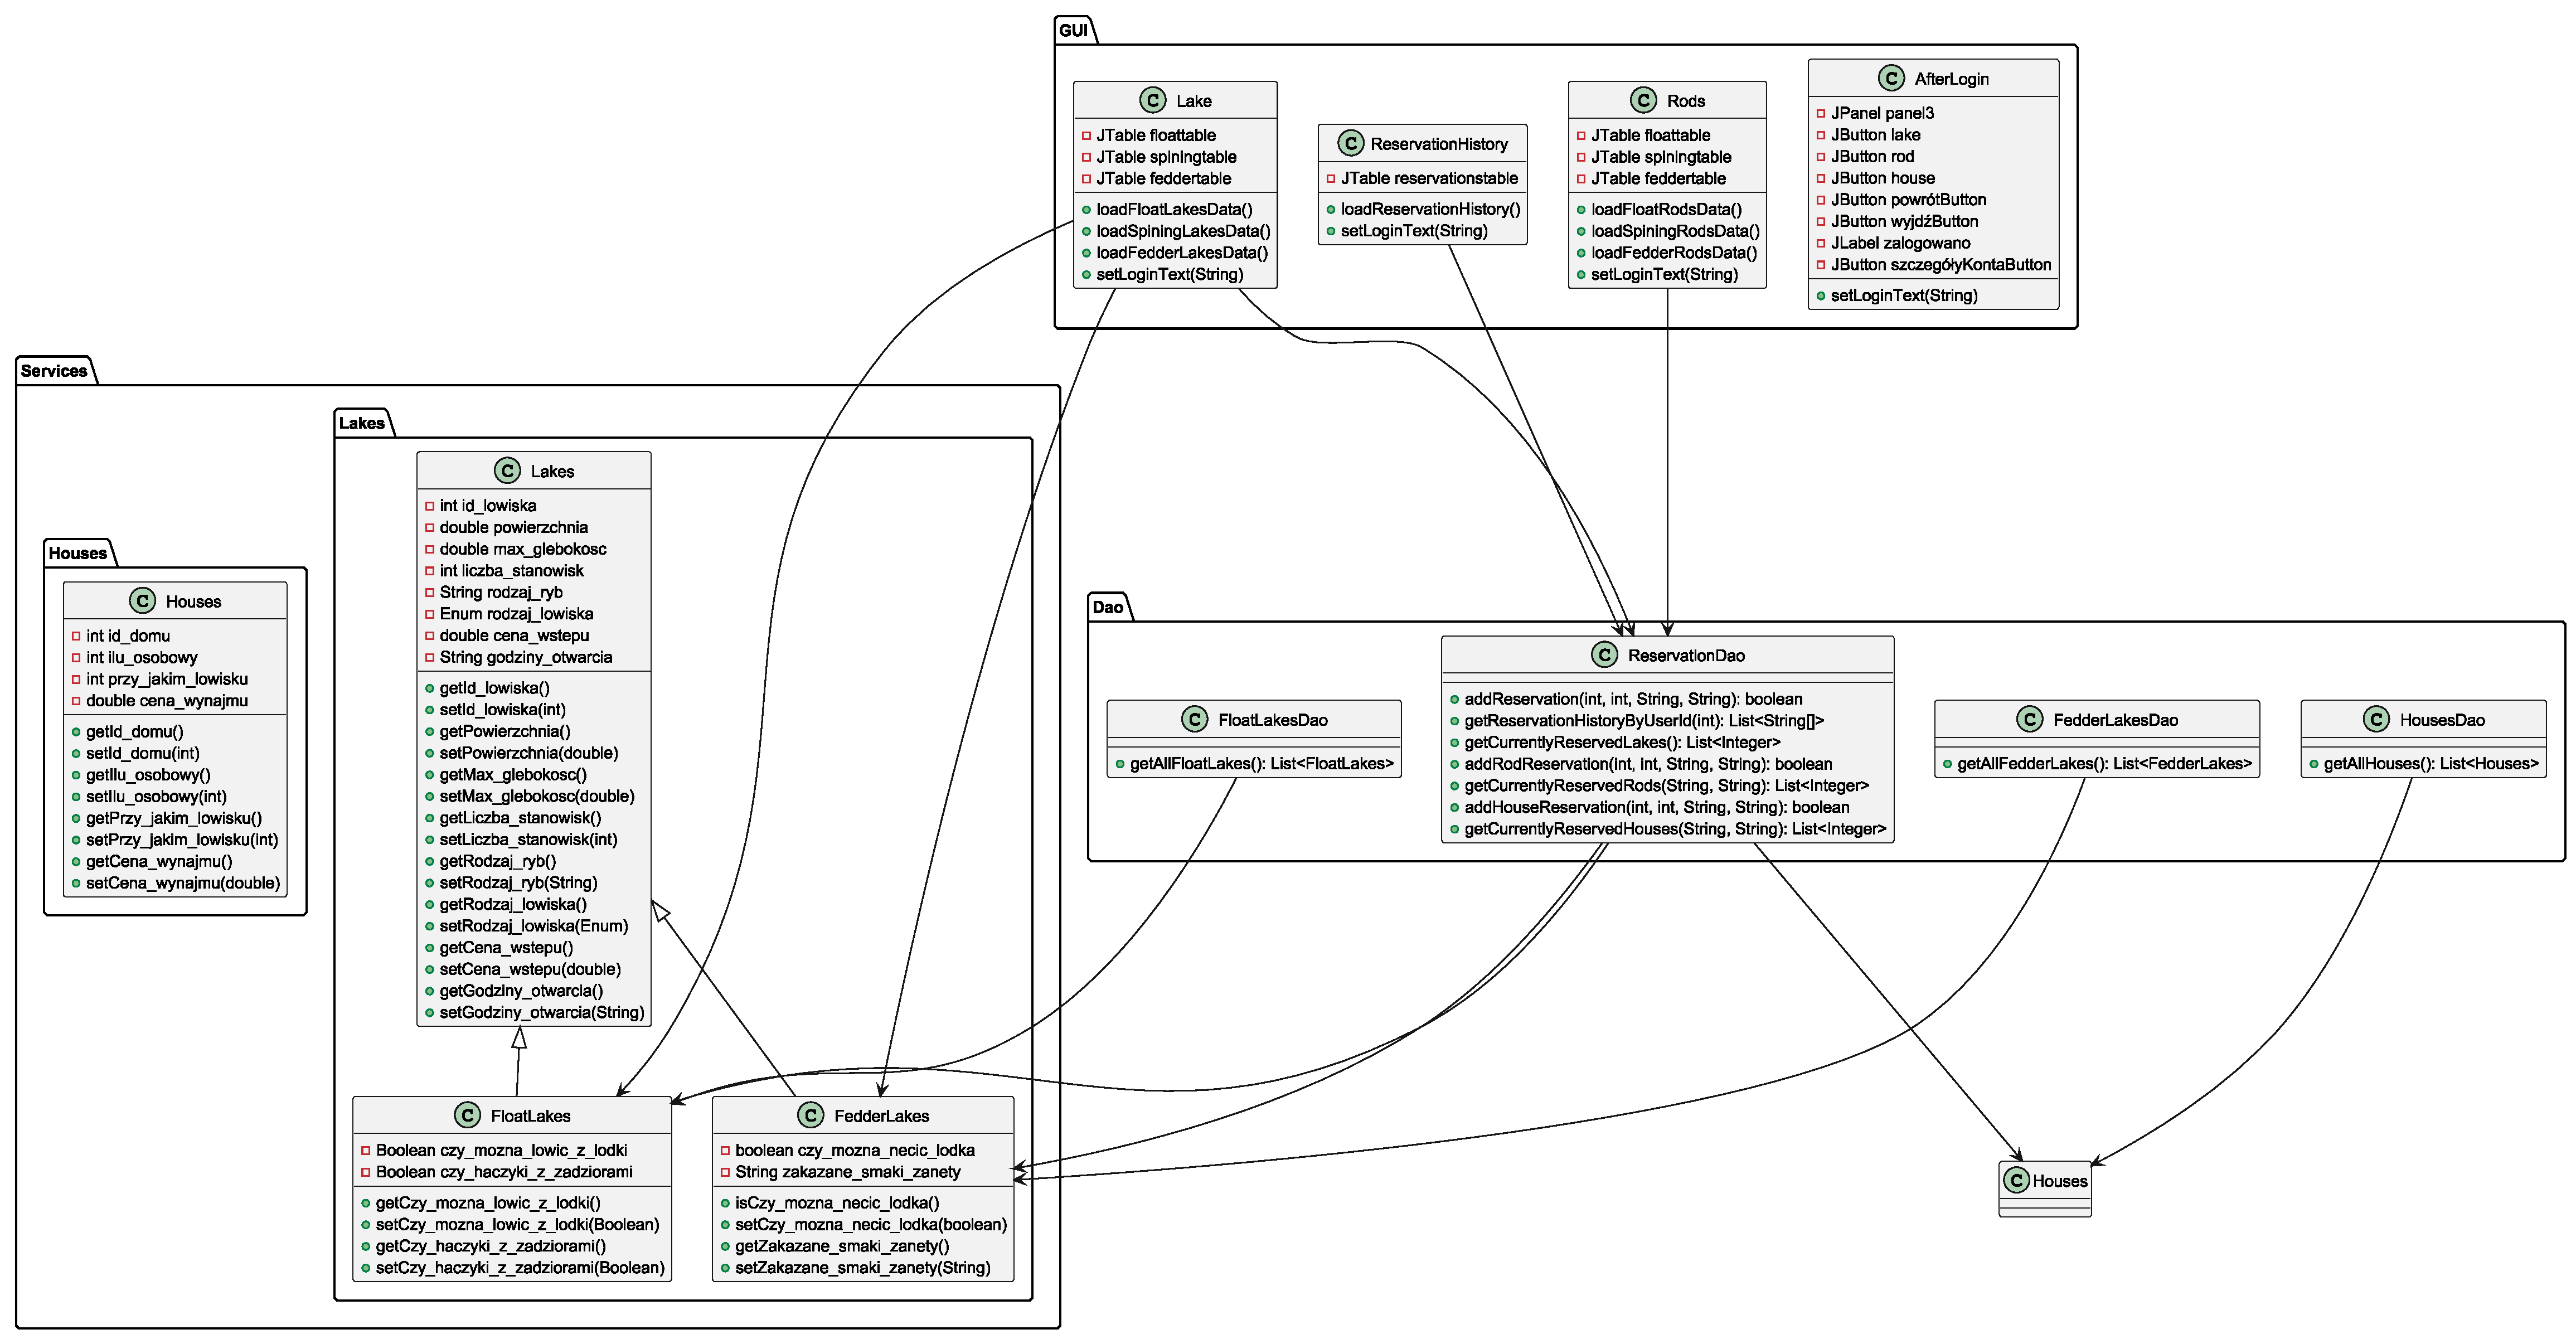
\includegraphics[width=1.1\linewidth]{figures/diagram.eps}
    \caption{Diagram klas UML projektu.}
    \label{fig:umldiagram}
    \small{Źródło: Opracowane przy użyciu PlantUML}
\end{figure}
\clearpage

\section{Zarządzanie danymi i baza danych lowisko}
\label{sec:baza_danych_nowe}
Baza danych MySQL jest kluczowym elementem projektu, przechowującym wszystkie istotne informacje o użytkownikach, rezerwacjach, łowiskach i innych zasobach. Struktura bazy danych została zaprojektowana w sposób umożliwiający łatwe zarządzanie danymi oraz ich efektywne przetwarzanie.
Baza danych składa się z kilku tabel, które są ze sobą powiązane relacjami. Schemat bazy danych (Rys. \ref{fig:erddiagram}) przedstawia strukturę tabel oraz ich relacje. 
\begin{figure}[H]
    \centering
    
\includegraphics[width=\linewidth]{figures/dbd.eps}
    \caption{Schemat bazy danych (ERD) łowiska wędkarskiego.}
    \label{fig:erddiagram}
    \small{Źródło: Wygenerowano za pomocą https://drawsql.app}
\end{figure}
\clearpage

\section{Wymagania systemowe i narzędzia do uruchomienia projektu}
Aby uruchomić projekt, wymagane są następujące narzędzia i oprogramowanie:
\begin{itemize}
    \item \textbf{Pakiet XAMPP:} Jest to pakiet oprogramowania, który zawiera serwer Apache, MySQL oraz PHP. Jest niezbędny do uruchomienia bazy danych MySQL, która jest kluczowym elementem projektu.
    \item \textbf{Środowisko IntelliJ IDEA:} Jest to zintegrowane środowisko programistyczne (IDE) dla języka Java, w którym projekt został stworzony. IntelliJ IDEA oferuje zaawansowane funkcje, takie jak automatyczne uzupełnianie kodu, refaktoryzacja i debugowanie, co znacznie ułatwia pracę programisty. 
    \item \textbf{Java Development Kit (JDK):} Wersja JDK 17 lub nowsza jest wymagana do kompilacji i uruchomienia aplikacji. JDK zawiera wszystkie niezbędne biblioteki i narzędzia do pracy z językiem Java.
    \item \textbf{MySQL Connector/J:} Jest to sterownik JDBC dla MySQL, który umożliwia aplikacji Java komunikację z bazą danych MySQL. Należy go dodać do project structure w modułach w projekcie IntelliJ IDEA.
\end{itemize}

    



\chapter{Harmonogram realizacji projektu.}
\label{chap:harmonogram}

\section{Harmonogram realizacji projektu. - Diagram Gantta}
Harmonogram realizacji projektu jest kluczowym elementem planowania, który pozwala na efektywne zarządzanie czasem i zasobami. W projekcie dotyczącym systemu rezerwacji usług łowiska wędkarskiego, harmonogram został opracowany z uwzględnieniem wszystkich istotnych etapów, od analizy wymagań po testowanie i wdrożenie.
\begin {itemize}
    \item \textbf{Analiza wymagań:} Zbieranie i analiza wymagań funkcjonalnych i niefunkcjonalnych systemu.
    \item \textbf{Projektowanie architektury:} Opracowanie struktury projektu, w tym diagramów UML i schematu bazy danych.
    \item \textbf{Implementacja:} Programowanie poszczególnych komponentów systemu, takich jak warstwa dostępu do danych, logika biznesowa i interfejs użytkownika.
    \item \textbf{Testowanie i dokumentacja:} Przeprowadzenie testów jednostkowych i integracyjnych, a także przygotowanie dokumentacji użytkownika i technicznej.
\end{itemize}

\begin{figure}[H]
    \centering
    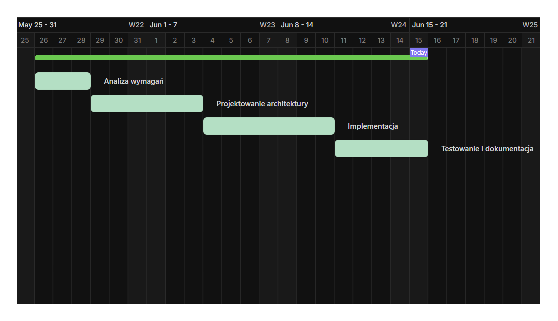
\includegraphics[width=\linewidth]{figures/gantt.eps}
    \caption{Harmonogram realizacji projektu (Diagram Gantta).}
    \label{fig:gantt_chart}
    \small{Źródło: Wygenerowano za pomocą https://clickup.com}
\end{figure}

\section{System kontroli wersji i repozytorium}
W projekcie zastosowano system kontroli wersji Git, który umożliwia śledzenie zmian w kodzie źródłowym, zarządzanie wersjami oraz współpracę zespołową. Git pozwala na tworzenie gałęzi (branch), co umożliwia równoległe prace nad różnymi funkcjonalnościami bez wpływu na główną linię rozwoju projektu.

Jako centralne, zdalne repozytorium kodu wykorzystano platformę GitHub. Cały projekt jest publicznie dostępny pod adresem:
\begin{center}
    \url{https://github.com/KamilKopczyk/Projekt_PO_JAVA_Kamil_Kopczyk_134927}
\end{center}





\include{chapters/5_Prezentacja_warstwy_użytkowej_projektu}
\chapter{Testowanie okienek błędów i innych elementów GUI}
\label{chap:testowanie}

\section{Wprowadzenie}
W tym rozdziale zostaną przedstawione testy przeprowadzone na okienkach błędów oraz innych elementach graficznego interfejsu użytkownika (GUI) aplikacji. Testowanie GUI jest kluczowym etapem w procesie tworzenia oprogramowania, ponieważ pozwala na identyfikację i naprawę błędów, które mogą wpływać na doświadczenie użytkownika.

\section{Okienka ostrzegawcze ekranu logowania}
Okienka ostrzegawcze na ekranie logowania są istotnym elementem interfejsu użytkownika, który informuje o błędach wprowadzonych danych. Testy te mają na celu sprawdzenie, czy okienka poprawnie reagują na nieprawidłowe dane wejściowe.
\begin{figure}[H]
    \centering
    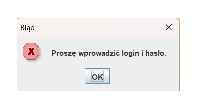
\includegraphics[width=0.8\linewidth]{figures/l1.eps}
    \caption{Brak danych w polach logowania.}
    \label{fig:login_win}
    \small{Źródło: Opracowane przy użyciu Java Swing}
\end{figure}
\clearpage

Podczas testów sprawdzano czy jak ktoś wpisze błędne dane logowania to czy pyta go czy chce się zarejestrować, czy kontynuować logowanie.

\begin{figure}[H]
    \centering
    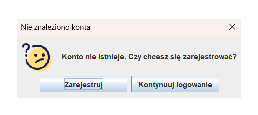
\includegraphics[width=0.8\linewidth]{figures/l2.eps}
    \caption{Błędne dane logowania.}
    \label{fig:login_win}
    \small{Źródło: Opracowane przy użyciu Java Swing}
\end{figure}
\clearpage

\section{Okienka ostrzegawcze ekranu rejestracjii}
Okienka ostrzegawcze na ekranie rejestracji informują użytkownika o błędach wprowadzonych danych podczas tworzenia nowego konta. Testy te mają na celu sprawdzenie, czy aplikacja poprawnie reaguje na nieprawidłowe dane wejściowe, takie jak brak wymaganych pól lub nieprawidłowy format danych.

\begin{figure}[H]
    \centering
    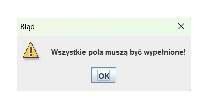
\includegraphics[width=0.8\linewidth]{figures/r1.eps}
    \caption{Brak danych w polach rejestracji.}
    \label{fig:register_win}
    \small{Źródło: Opracowane przy użyciu Java Swing}
\end{figure}
\clearpage

\begin{figure}[H]
    \centering
    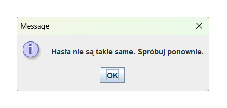
\includegraphics[width=0.8\linewidth]{figures/r2.eps}
    \caption{Sprawdzanie czy hasła są identyczne.}
    \label{fig:register_win}
    \small{Źródło: Opracowane przy użyciu Java Swing}
    \end{figure}
\clearpage

\begin{figure}[H]
    \centering  
    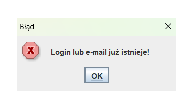
\includegraphics[width=0.8\linewidth]{figures/r3.eps}
    \caption{Sprawdzanie czy login lub e-mail nie są już przez kogoś używane.}
    \label{fig:register_win}
    \small{Źródło: Opracowane przy użyciu Java Swing}
    \end{figure}
\clearpage

\section {Okienka ostrzegawcze ekranu rezerwacji}
Okienka ostrzegawcze na ekranie rezerwacji informują użytkownika o błędach związanych z rezerwacją, takich jak nieprawidłowy format daty lub próba dokonania rezerwacji w przeszłości. Testy te mają na celu sprawdzenie, czy aplikacja poprawnie reaguje na nieprawidłowe dane wejściowe i czy informuje użytkownika o konieczności wprowadzenia poprawnych danych.
\begin{figure}[H]
    \centering
    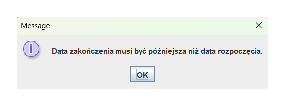
\includegraphics[width=0.8\linewidth]{figures/r4.eps}
    \caption{Data startu rezerwacji jest późniejsza niż końca rezerwacji.}
    \label{fig:reservation_win}
    \small{Źródło: Opracowane przy użyciu Java Swing}
\end{figure}
\clearpage

\begin{figure}[H]
    \centering
    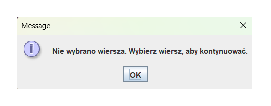
\includegraphics[width=0.8\linewidth]{figures/r5.eps}
    \caption{Nie wybranie wiersza do rezerwacji.}
    \label{fig:reservation_win}
    \small{Źródło: Opracowane przy użyciu Java Swing}   
\end{figure}
\clearpage

\section{Okienka ostrzegawcze ekranu rezerwacji i histori bez logowania}
Okienka ostrzegawcze na ekranie rezerwacji bez logowania informują użytkownika o konieczności zalogowania się, aby móc dokonać rezerwacji. Testy te mają na celu sprawdzenie, czy aplikacja poprawnie reaguje na próby dokonania rezerwacji przez niezalogowanych użytkowników i czy informuje ich o konieczności zalogowania się.

\begin{figure}[H]
    \centering
    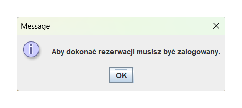
\includegraphics[width=0.8\linewidth]{figures/r6.eps}
    \caption{Próba rezerwacji bez zalogowania.}
    \label{fig:reservation_win}
    \small{Źródło: Opracowane przy użyciu Java Swing}
\end{figure}
\clearpage

\begin{figure}[H]
    \centering
    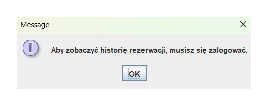
\includegraphics[width=0.8\linewidth]{figures/r7.eps}
    \caption{Próba sprawdzenia historii rezerwacji bez zalogowania.}
    \label{fig:reservation_win}
    \small{Źródło: Opracowane przy użyciu Java Swing}
\end{figure}
\clearpage





\chapter{Podsumowanie}
\label{chap:podsumowanie}

\section{Wnioski}
Projekt systemu rezerwacji usług łowiska wędkarskiego został zrealizowany zgodnie z założeniami i wymaganiami określonymi na początku prac. Aplikacja umożliwia użytkownikom łatwe zarządzanie rezerwacjami łowisk, wędek i domków, a także zapewnia intuicyjny interfejs graficzny.
Zastosowanie technologii Java oraz biblioteki Swing pozwoliło na stworzenie aplikacji, która jest zarówno funkcjonalna, jak i estetyczna. System został zaprojektowany z myślą o wydajności, bezpieczeństwie i łatwości obsługi, co zostało osiągnięte poprzez odpowiednią strukturę kodu.
\section{Przyszłe kierunki rozwoju}
W przyszłości planowane jest rozszerzenie funkcjonalności aplikacji o dodatkowe usługi, takie jak estetyczniejsze wybory dat, możliwość dodawania opinii o łowiskach i domkach.
Dodatkow rozważane jest wprowadzenie możliwości resetowania hasła przez użytkowników, co zwiększy bezpieczeństwo i wygodę korzystania z aplikacji.




\renewcommand{\emph}[1]{\uline{#1}}

\clearpage
% Dodanie spisu rysunków do spisu treści
\addcontentsline{toc}{section}{\textbf{Spis rysunków}}
\listoffigures
\clearpage


% \appendix
\chapter*{}
\label{cha:statement-A}


\begin{figure}[H]
    \centering
    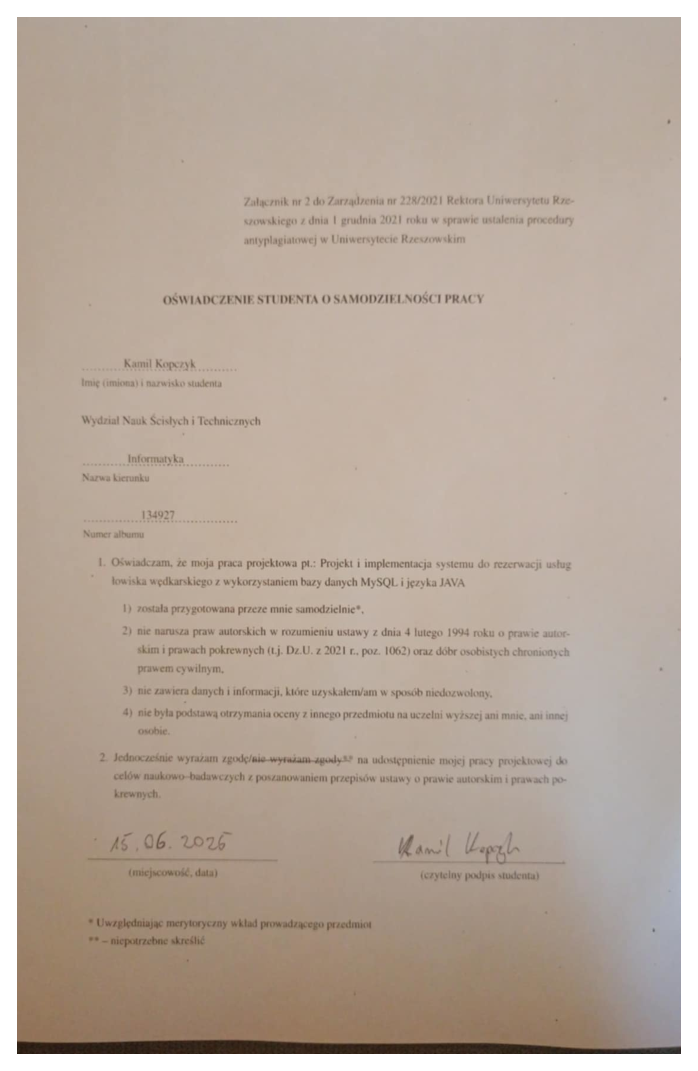
\includegraphics[width=0.8\linewidth]{figures/oswiadczenie.eps}
    \caption{Oświadczenie o samodzielnym wykonaniu projektu.}
    \label{fig:statementA}
\end{figure}
\clearpage

\end{document}
